\documentclass[border=4pt]{standalone}
\usepackage{amsmath,amssymb,bm}
\usepackage{tikz}
\usetikzlibrary{arrows.meta,positioning,fit,backgrounds,calc,shapes.geometric}

\begin{document}
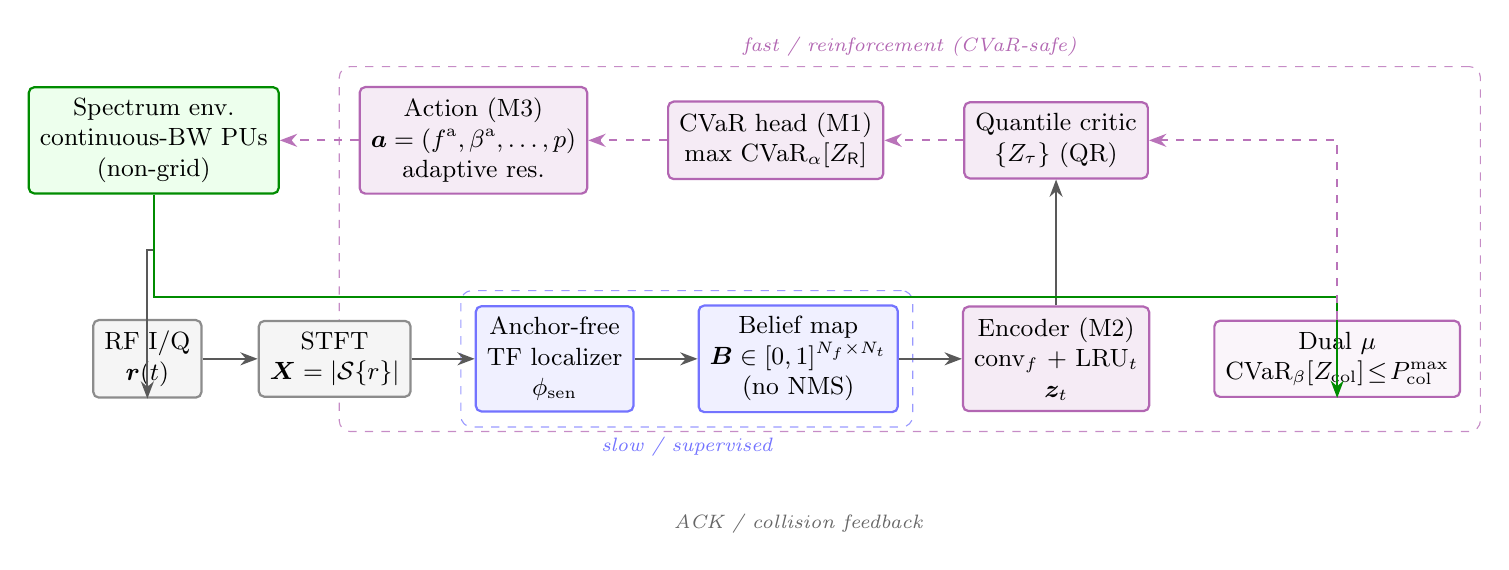
\begin{tikzpicture}[
  font=\small,
  >={Stealth[length=2.2mm]},
  block/.style={rectangle, rounded corners=2pt, draw=black!70, thick,
                align=center, minimum height=9mm, inner sep=4pt, fill=white},
  sens/.style={block, fill=blue!6, draw=blue!55},
  acc/.style={block, fill=violet!8, draw=violet!60},
  io/.style={block, fill=black!4, draw=black!45},
  env/.style={block, fill=green!7, draw=green!55!black},
  lbl/.style={font=\scriptsize\itshape, text=black!60},
  ar/.style={->, thick, draw=black!65},
  arb/.style={->, thick, draw=violet!55, dashed},
]

% ---------- bottom: signal -> spectrogram ----------
\node[io] (rx) {RF I/Q\\$\bm{r}(t)$};
\node[io, right=7mm of rx] (stft) {STFT\\$\bm{X}=|\mathcal{S}\{r\}|$};

% ---------- sensing tier ----------
\node[sens, right=8mm of stft] (det) {Anchor-free\\TF localizer\\$\phi_{\mathrm{sen}}$};
\node[sens, right=8mm of det] (bel) {Belief map\\$\bm{B}\in[0,1]^{N_f\times N_t}$\\(no NMS)};

% ---------- state encoder (M2) ----------
\node[acc, right=8mm of bel] (enc) {Encoder (M2)\\conv$_f$ + LRU$_t$\\$\bm{z}_t$};

% ---------- access tier (M1) : place above ----------
\node[acc, above=16mm of enc] (critic) {Quantile critic\\$\{Z_\tau\}$ (QR)};
\node[acc, left=10mm of critic] (head) {CVaR head (M1)\\$\max\,\mathrm{CVaR}_\alpha[Z_{\mathsf{R}}]$};
\node[acc, left=10mm of head] (act) {Action (M3)\\$\bm{a}=(f^{\mathrm a},\beta^{\mathrm a},\dots,p)$\\adaptive res.};

% ---------- environment / feedback ----------
\node[env, left=10mm of act] (envb) {Spectrum env.\\continuous-BW PUs\\(non-grid)};

% ---------- dual control (right margin, between rows) ----------
\node[acc, right=8mm of enc, fill=violet!4] (dual)
  {Dual $\mu$\\$\mathrm{CVaR}_\beta[Z_{\mathrm{col}}]\!\le\!P_{\mathrm{col}}^{\max}$};

% ===== forward edges (bottom row L->R) =====
\draw[ar] (rx) -- (stft);
\draw[ar] (stft) -- (det);
\draw[ar] (det) -- (bel);
\draw[ar] (bel) -- (enc);
\draw[ar] (enc) -- (critic);

% ===== access loop (top row R->L) =====
\draw[arb] (critic) -- (head);
\draw[arb] (head) -- (act);
\draw[arb] (act) -- (envb);

% ===== environment back to sensing: route along far left, below =====
\draw[ar] (envb.south) -- ++(0,-7mm) -| (rx.south);

% ===== ACK / collision feedback to dual, then dual to critic =====
\draw[ar, draw=green!55!black] (envb.south) -- ++(0,-13mm) -| (dual.south);
\node[lbl, below=11.5mm of bel] {ACK / collision feedback};
\draw[arb] (dual.north) |- (critic.east);

% ===== timescale annotations =====
\begin{scope}[on background layer]
  \node[draw=blue!40, dashed, rounded corners, fit=(det)(bel),
        inner sep=5pt, label={[lbl, blue!55]below:slow / supervised}] {};
  \node[draw=violet!45, dashed, rounded corners,
        fit=(enc)(critic)(head)(act)(dual),
        inner sep=7pt, label={[lbl, violet!60]above:fast / reinforcement (CVaR-safe)}] {};
\end{scope}

\end{tikzpicture}
\end{document}
